
%% <<아래한글 기준>>
%% - 편집용지 : A4(210 x 297mm)
%% - 용지여백 : 위 · 아래 여백 38mm, 머리말 · 꼬리말 15mm
%%              좌 · 우 여백 35mm
%% - 들여쓰기 : 문단 시작은 2칸 띄움
%% - 줄 간 격 : 160% - 200%
%% - 정렬방식 : 혼합
%% - 글씨체 및 크기
%%   · 큰 제 목 - 16point (명조, 신명조, 바탕체, 굴림체 중 사용), 진하게
%%   · 중간제목 - 13point (명조, 신명조, 바탕체, 굴림체 중 사용), 진하게
%%   · 본    문 - 10 또는 11point (명조, 신명조, 바탕체, 굴림체 중 사용)
%%   · 각    주 - 9point (명조, 신명조, 바탕체, 굴림체 중 사용)
%%
%%
%% <<학위논문 제본방법>>
%% 1. 판  종 : 4ㆍ6배판(18.5cm X 25.5cm)
%% 2. 지  질 : 70파운드 이상 모조지
%% 3. 인쇄방식 : 단면 혹은 양면 인쇄하되 논문은 마스터, 옵셋인쇄로 한다.
%% 4. 제 본 식 : 클로스 양장. 다만, 석사학위논문에 한해 클로스 양장 또는 종이제본 중 어느 것으로도 할 수 있다.
%% 5. 표지색깔 : 석사학위논문은 진한 감(紺)색, 박사학위논문은 흑(黑)색으로 한다. 석사학위 논문을 종이 제본하는 경우에는 회백색으로 한다.
%% 6. 표지인쇄방식 : 다음 [그림 1]에 따르며, 명조체 2호(22p) 활자로 하고 금색으로 인쇄한다. 석사학위논문을 종이 제본하는 경우에는 회백색으로 한다.
%%


\documentclass[a4paper,         % 공급용지
                11pt,           % 본문 글씨 크기
                oneside,        % 단면 인쇄
                openany,        % 임의의 챕터 시작 페이지
                % chapter,        %
                % draft,
                showtrims       % 재단선 표시
                ]{oblivoir}     %


%% 편집용지 지정
\usepackage{fapapersize}
\usefapapersize{*,*,35mm,*,53mm,*}

%% 머리말 꼬리말 높이 지정. \usefapapersize 이후에 지정할 수 있음.
\setheadfoot{15mm}{15mm}
\setheaderspaces{*}{0pt}{*}


\usepackage{listings}
\usepackage{amsmath}
% 표의 row 간격 조절에 사용하는 변수값도 \arraystretch로 같아서,
% 매트릭스일 경우만 \arraystretch를 다시 1.0으로 설정하도록 지정.
\makeatletter
\renewcommand*\env@matrix{ %
    \edef\arraystretch{0.7} %
    \hskip -\arraycolsep
    \let\@ifnextchar\new@ifnextchar
    \array{*\c@MaxMatrixCols c}}
\makeatother

\let\comment\undefined
\let\added\undefined
\let\deleted\undefined
\usepackage{changes}
\definechangesauthor[name={Delete}, color=red]{del}
\definechangesauthor[name={Add}, color=blue]{add}
\definechangesauthor[name={Note}, color=orange]{note}
\definechangesauthor[name={Yoo}, color=green]{yoo}
\setauthormarkuptext{}
\newcommand{\add}[1]{\added[id=add]{#1}}
\newcommand{\del}[1]{\deleted[id=del]{#1}}
\newcommand{\repl}[2]{\added[id=add]{#1}\deleted[id=del]{#2}}

\usepackage[singlelinecheck=true]{caption}
% 출처용 캡션의 글씨 크기만 줄임.
\makeatletter
\patchcmd{\caption@@@make}% <cmd>
  {\ifcaption@star}% <search>
    {\ifcaption@star\scriptsize}% <replace>
    {}{}% <success><failure>
\makeatother
\usepackage[labelformat=simple]{subcaption}
\usepackage{tabularx}
% subfigure를 레퍼런스할 때 괄호 포매팅이 되도록 지정
\renewcommand\thesubfigure{(\alph{subfigure})}
% 자간 조정
% \usepackage[letterspace=125]{microtype}


\let\printglossary\relax
\let\theglossary\relax
\let\endtheglossary\relax
\usepackage[acronym, toc, section, nogroupskip, style=index]{glossaries}
\usepackage{pdfpages}

\newcommand{\urlfootnote}[1]{\protect\footnote{\url{#1}}}

\usepackage[backend=biber,style=numeric,maxnames=100,sorting=none]{biblatex}
\addbibresource{reference.bib}
\renewcommand{\finalnamedelim}{, }

\usepackage{rotating}


\usepackage{graphicx}
\usepackage{epsfig}
\usepackage{fancyhdr}
\usepackage{environ}
\usepackage{siunitx}


\usepackage{yonseiThesis} 


%%%%%%%%%%%%%%%%%%%%%%%%%%%%%%%%%%%%%%%%%%%%%%%%%%%%%%%%%%%%%
% 들여쓰기 1em
\setlength{\parindent}{1em}


\hypersetup{
    hidelinks
}

\usepackage{multirow}

% 표 column 간격 조절
\setlength{\tabcolsep}{8px}
% 표 row 간격 조절
\renewcommand{\arraystretch}{1.8}


% makeglossaries 커맨드가 main.tex에 있어야 함...
\makeglossaries

% 선언된 약호들은 실제로 본문에서 인용되어야 약호표에 노출됨.

\newacronym{lidar}{LiDAR}{Light Detection And Ranging}
\newacronym{fov}{FoV}{Field of View}
\newacronym{cscw}{CSCW}{Computer-Supported Cooperative Work}
\newacronym{ui}{UI}{User Interface}
\newacronym{gpgpu}{GPGPU}{General Purpose computing on Graphic Processing Unit}
\newacronym{cpu}{CPU}{Central Processing Unit}
\newacronym{http}{HTTP}{HyperText Transfer Protocol}
\newacronym{p2p}{P2P}{Peer-To-Peer}
\newacronym{webrtc}{WebRTC}{Web Real-Time Communication}
\newacronym{cve}{CVE}{Collaborative virtual environment}
\newacronym{cave}{CAVE}{Cave Automatic Virtual Environment}
\newacronym{hmd}{HMD}{Head-Mounted Device}
\newacronym{xr}{XR}{Extended Reality}
\newacronym{svr}{SVR}{Spatial Virtual Reality}
\newacronym{sar}{SAR}{Spatial Augmented Reality}
\newacronym{ir}{IR}{Infra Red}
\newacronym{ogc}{OGC}{Open Geospatial Consortium}
\newacronym{arml}{ARML}{Augmented Reality Markup Language }
\newacronym{gml}{GML}{Geography Markup Language}
\newacronym{kml}{KML}{Keyhole Markup Language}
\newacronym{x3d}{X3D}{Extensible 3D}
\newacronym{vrml}{VRML}{Virtual Reality Markup Language}
\newacronym{vrpn}{VRPN}{Virtual Reality Peripheral Network}
\newacronym{ict}{ICT}{Information and communications technology}
\newacronym{voip}{VoIP}{Voice over Internet Protocol}
\newacronym{vr}{VR}{Virtual Reality}
\newacronym{ar}{AR}{Augmented Reality}
\newacronym{lng}{LNG}{Liquefied Natural Gas}
\newacronym{xml}{XML}{Extensible Markup Language}
\newacronym{html}{HTML}{HyperText Markup Language}
\newacronym{dom}{DOM}{Document Object Model}
\newacronym{css}{CSS}{Cascading Style Sheets}
\newacronym{ajax}{Ajax}{Asynchronous JavaScript and XML}
\newacronym{url}{URL}{Uniform Resource Locator}
\newacronym{sdp}{SDP}{Session Description Protocol}
\newacronym{ice}{ICE}{Interactive Connectivity Establishment}
\newacronym{ip}{IP}{Internet Protocol}
\newacronym{stun}{STUN}{Session Traversal Utilities for NAT}
\newacronym{turn}{TURN}{Traversal Using Relays around NAT}
\newacronym{nat}{NAT}{Network Address Translation}
\newacronym{ooi}{OOI}{Object of Interest}
\newacronym{dof}{DOF}{Degrees of Freedom}
\newacronym{iot}{IoT}{Internet of Things}
\newacronym{ge}{GE}{General Electric}
\newacronym{w3c}{W3C}{World Wide Web Consortium}
\newacronym{slam}{SLAM}{Simultaneous Localization And Mapping}
\newacronym{wxr}{WXR}{Webized XR}
\newacronym{udp}{UDP}{User Datagram Protocol}
\newacronym{tcp}{TCP}{Transmission Control Protocol}
\newacronym{plm}{PLM}{Product Lifecycle Management}
\newacronym{lan}{LAN}{Local Area Network}



% 메타데이터
\titleEng{Web-based Remote XR Collaboration \\ Using Real-time Digital Twinning of Workspace}
\titleKr{실시간 디지털 트윈 공간 구성을 이용한 \\ 웹 기반 원격 XR 협업 방법}
\authorNameEng{Yongjae Lee}
\authorNameKr{이용재}
\affilDeptNameEng{Dept. of Mechanical Engineering}
\affilDeptNameKr{기계공학과}
\affilSchoolNameEng{The Graduate School}
\affilSchoolNameKr{대학원}
\affilUnivNameEng{Yonsei University}
\affilUnivNameKr{연세대학교}
\advisor{이수홍}{유병현}
\submitDate{2021년 7월 9일}

% 인준서
% 다음 라인을 주석처리하면 서명란이 비어있는 페이지가 생성됨.
\approvalFile{approval.pdf}
\approvalDate{2021년 7월 9일}



\acknowledgement{
감사의 말 감사의 말 감사의 말 감사의 말 감사의 말 감사의 말 감사의 말 감사의 말 감사의 말 감사의 말 감사의 말 감사의 말 감사의 말 감사의 말 감사의 말 감사의 말 감사의 말 감사의 말 감사의 말 감사의 말 감사의 말 감사의 말 감사의 말 감사의 말 감사의 말 감사의 말 감사의 말 감사의 말 감사의 말 감사의 말 감사의 말 감사의 말 감사의 말 감사의 말 감사의 말 감사의 말 감사의 말 감사의 말 감사의 말 감사의 말 감사의 말 감사의 말 감사의 말 감사의 말 감사의 말 감사의 말 감사의 말 감사의 말 감사의 말 감사의 말
}

\acknowledgementDate{2021년 7월}

\abstractKr{

원격 협업 기술은 작업자들이 물리적으로 한곳에 모이지 않고도 협업할 수 있게 만들어 주었으며, 작업자들은 협업하기 위해 먼 거리를 이동하지 않아도 되므로 시간 및 비용을 절약할 수 있게 되었다. 근래의 원격 협업은 단순한 화상회의를 넘어 가상현실(\acrshort{vr})과 증강현실(\acrshort{ar})을 활용하는 확장현실(\acrshort{xr}) 기술을 통해 이루어지고 있다. \acrshort{ar}을 이용한 원격 협업은 현장 작업자의 카메라 뷰가 공유되고 원격지의 작업자가 음성 또는 드로잉 등을 통해 작업 지시를 전달하는 방식으로 이루어진다. 이때, 원격 작업자는 현장을 관찰하는 시점을 자유롭게 바꾸지 못하고 현장 작업자의 카메라 움직임에 의존하여 수동적으로 현장의 상황을 파악하게 되어 협업이 더디게 이루어진다. 다른 방식의 \acrshort{xr} 협업으로, 원격 작업자가 좀 더 몰입적인 환경에서 현장을 체험할 수 있도록 현장을 3차원 재구성한 디지털 트윈 공간에서 협업을 진행하는 방법이 있다. 하지만, 현장에 많은 센서를 설치하거나 또는, 현장을 본뜬 3D 모델을 만드는 등 부가적인 작업이 많아 이 방법 또한 실용적이지 못하였다.

본 연구의 `실시간 디지털 트윈 공간 구성을 이용한 웹 기반 원격 \acrshort{xr} 협업 방법'은 협업 대상과 배경 공간을 구분하여, 협업 대상만 사전에 3D 모델링을 하고 배경은 협업을 할 때 현장에서 실시간으로 재구성하는 방식의 협업을 제안한다. 이 방법은 협업을 위한 3D 모델링 작업을 최소화하고 센서 설치를 필요로 하지 않아 기존 방법보다 실용적인 \acrshort{xr} 협업 경험을 제공한다. 본 연구는 두 개의 하위 기술로 나뉜다. `웹 기반의 원격 \acrshort{xr} 협업'은 이미지 트래킹 기술을 이용해 협업 대상의 위치를 추적하고 추적한 위치 정보를 원격 작업자에게 동기화한다. 이때, 획득한 물체의 위치는 카메라 좌표계에서 상에서 정의되는데 이를 원격 작업자가 사용하는 월드 좌표계로 변환하기 위해 `스페이스 마커'를 도입하였다. 그리고, 원격 작업자와 현장 작업자가 각각 이용하는 \acrshort{vr} 콘텐츠와 \acrshort{ar} 콘텐츠를 한 번에 표현할 수 있는 \acrshort{xr} 콘텐츠 표현을 정의하여 동일한 협업 시나리오에 대해 중복적인 콘텐츠를 생성하지 않아도 되도록 만들었다. `실시간 디지털 트윈 공간 구성'은 \acrshort{lidar} 센서를 이용하여 현장의 깊이 데이터를 수집하고 핀홀 카메라 모델을 통해 포인트 클라우드 데이터로 3차원 재구성한다. 재구성한 포인트 클라우드 데이터에서 협업 대상에 해당하는 부분은 마스킹하여 제거하고 웹 표준의 \acrshort{p2p} 통신 기술인 \acrshort{webrtc}를 이용하여 원격 작업자에게 전달한다. 원격 작업자는 전달받은 포인트 클라우드 데이터를 누적하여 현장을 복제한 디지털 트윈 공간을 구성하고, 이를 통해 더욱 직관적으로 현장의 상황을 파악할 수 있게 된다. 현장 작업자는 단순한 드로잉이 아닌 3D 모델을 협업 대상 위에 겹쳐 봄으로써 직관적으로 작업 정보를 파악할 수 있어 협업의 능률을 향상시킬 수 있다. 또한, 본 연구에서 제안하는 \acrshort{xr} 협업 방법은 사람 간의 협업뿐만 아니라 원격 로봇 조종 등과 같은 다양한 미래 산업 분야에도 응용될 수 있을 것으로 본다.

}


\abstractEng{

Remote collaboration technology has enabled workers to work together without physically gathering, saving time and money by not having to travel long distances to collaborate. Recent remote collaboration has been achieved through \acrfull{xr} that leverage \acrfull{vr} and \acrfull{ar}, beyond simple video conferencing. Remote collaboration using \acrshort{ar} takes place in such a way that local workers share their camera views and that remote workers communicate task instructions via voice or drawing on screen, etc. At this time, the remote worker cannot freely change the point of observing the site and relies on the camera movement of the local worker to grasp the situation of the site, which slows collaboration. In the other method of using \acrshort{xr}, there is a method to proceed collaboration in a three-dimensional reconstructed digital twin workspace where remote workers experience the local site in a more immersive environment. However, this method has also been impractical due to many additional tasks, such as installing many sensors in the local site, or creating 3D models replicating the local site.

In this work, we propose the method of `Web-based Remote \acrshort{xr} Collaboration Using Real-time Digital Twinning of Workspace' distinguishing collaboration targets and background spaces, in which only collaboration targets are 3D modeled in advance, and backgrounds are reconstructed in real-time. The method minimizes the 3D modeling task for collaboration and does not require sensor installation, providing a more practical \acrshort{xr} collaboration experience than previous methods. This study is divided into two sub-techniques. The `web-based remote \acrshort{xr} collaboration' uses image tracking techniques to track the pose of collaboration targets and synchronize the pose information to remote workers. Because the pose of tracked object is defined on the camera coordinate system, we introduced a `space marker' to transform it into a world coordinate system used by remote workers. In addition, we defined a \acrshort{xr} content representation method that can represent \acrshort{vr} content used by remote workers and \acrshort{ar} content used by local workers at once, eliminating the need to generate duplicate content for the same collaborative scenario. The `real-time digital twinning of workspace' technique collects depth data of the local site using a \acrshort{lidar} sensor and reconstructs them as point cloud data via pinhole camera models. Then, the parts corresponding to the collaboration target in the point cloud data are removed and sent to remote workers using \acrshort{webrtc}, a web standard communication technology. Remote workers construct digital twin spaces that replicate the local site by accumulating the delivered point cloud data, which allows them to more intuitively grasp the situation of the local site actually they did not visit. Also, local workers can intuitively grasp task instruction by watching the overlapped 3D models over collaborative targets rather than simple drawing on screen, which can improve collaboration efficiency. Furthermore, we believe that our proposed \acrshort{xr} collaboration method can be applied not only to human-to-human collaboration, but also to various industrial fields such as remote robot control.

}

\keywordsKr{확장현실, 가상현실, 증강현실, 웹 기반 확장현실, 원격 확장현실 협업, 실시간 디지털 트윈 공간 구성, 웹 기반 실시간 통신}
\keywordsEng{Extended Reality, XR, Virtual Reality, Augmented Reality, Web-based XR, Remote XR Collaboration, Real-time Digital Twinning, WebRTC}


\begin{document}

%% 머리지면 (preliminaries) 생성
\maketitlepages


    
\section{서론}
\subsection{연구의 배경}

\begin{figure}[h!]
    \centering
    \begin{subfigure}[t]{0.95\textwidth}
        \centering
        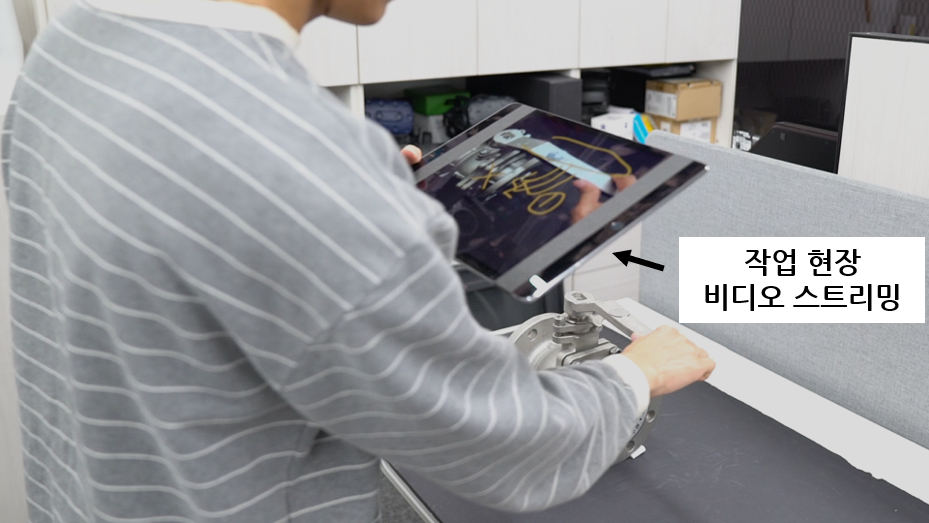
\includegraphics[width=\textwidth]{figures/remote_ar_local_site.png}
        \caption{현장 작업자의 모습: 작업 현장을 원격 작업자에게 비디오 스트리밍 하고 있음.}
        \label{fig:remote_ar_local_site}
    \end{subfigure}
    
    \par\bigskip
        
    \begin{subfigure}[t]{0.95\textwidth}
        \centering
        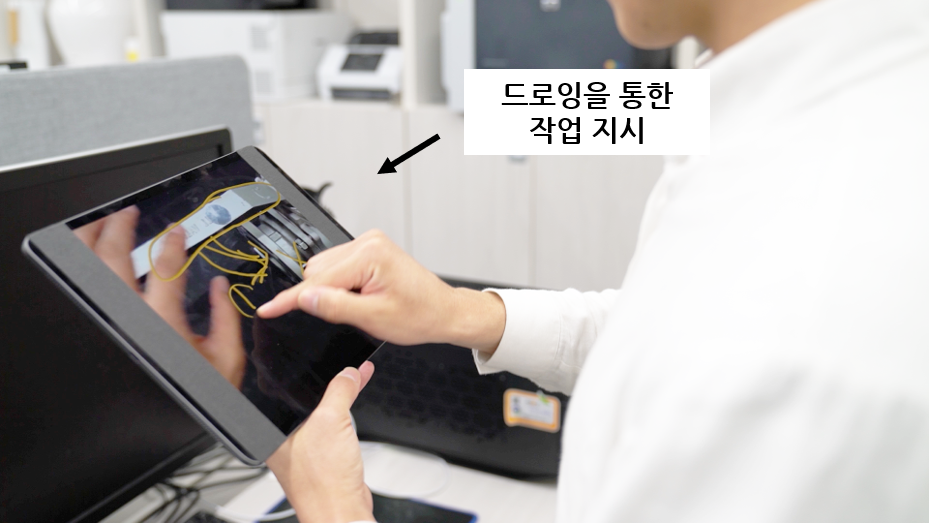
\includegraphics[width=\textwidth]{figures/remote_ar_remote_site.png}
        \caption{원격 작업자의 모습: 현장 작업자가 스트리밍하는 비디오를 통해 작업 현장의 상황을 파악하고, 그 위에 드로잉을 통해 현장 작업자가 해야될 작업을 지시하고 있음.}
        \label{fig:remote_ar_remote_site}
    \end{subfigure}
    \caption{원격 \acrshort{ar} 협업의 모습. 원격 \acrshort{ar} 협업은 원격 \acrshort{xr} 협업의 주류방식이 되었음.}
    \label{fig:remote_ar_collaobration_example}
\end{figure}


\subsection{연구의 목적}

\subsection{연구의 내용 및 구성}
    \newpage
    
    
\section{연구 동향 및 이론}
\subsection{디지털 트윈}

\subsection{XR 협업 기술}

\begin{sidewaystable}
\renewcommand{\arraystretch}{1.4}
\centering
\caption{XR 협업 연구의 예시 및 분류\cite{Lee2021XR}.}
\label{table:xr_coop_papers_table}

\begin{tabularx}{\textwidth}{cp{0.2\textwidth}X}
\hline
No.   & 타입 (Categories)                      & \multicolumn{1}{l}{참고문헌} \\ \hline
1     & Cooperation only on the virtual environment & Kato \& Billinghurst, 1999\cite{Kato1999Marker}; Shen \textit{et al.}, 2010\cite{Shen2010Augmented}; Wong \& Gutwin, 2014\cite{Wong2014Support}; Zillner \textit{et al.}, 2014\cite{Zillner20143D}; Higuch \textit{et al.}, 2015\cite{Higuch2015ImmerseBoard}; Müller \textit{et al.}, 2016\cite{Muller2016Virtual}; Dey \textit{et al.}, 2017\cite{Dey2017Effects}; Poretski \textit{et al.}, 2018\cite{Poretski2018Normative}; Grandi \textit{et al.}, 2019\cite{Grandi2019Characterizing}; Huh \textit{et al.}, 2019\cite{Huh2019XR}; Pereira \textit{et al.}, 2019\cite{Pereira2019Extended}      \\
2     & Spatial virtual reality                 & Beck \textit{et al.}, 2013\cite{Beck2013Immersive}; Febretti \textit{et al.}, 2013\cite{Febretti2013CAVE2}      \\
3     & Virtual collaboration interfaces        & Pauchet \textit{et al.}, 2007\cite{Pauchet2007Mutual}; Tang \textit{et al.}, 2010\cite{Tang2010Three}      \\ 
4     & Remote assistant AR (RGB)               & Lipson \textit{et al.}, 1998\cite{lipson1998online}; Bauer \textit{et al.}, 1999\cite{Bauer1999Where}; Gurevich \textit{et al.}, 2012\cite{Gurevich2012TeleAdvisor}; Kasahara \textit{et al.}, 2012\cite{Kasahara2012Second}; Gauglitz \textit{et al.}, 2014\cite{Gauglitz2014InTouch}; Kim \textit{et al.}, 2014\cite{Kim2014Improving}; Fakourfar \textit{et al.}, 2016\cite{Fakourfar2016Stabilized}; Gupta \textit{et al.}, 2016\cite{Gupta2016Do}; Nuernberger \textit{et al.}, 2016\cite{Nuernberger2016Anchoring}       \\
5     & Remote assistant AR (360)               & Chen \textit{et al.}, 2015\cite{Chen20153D}; Kratz \textit{et al.}, 2015\cite{Kratz2015Polly}; Nagai \textit{et al.}, 2015\cite{Nagai2015LiveSphere}; Kasahara \textit{et al.}, 2017\cite{Kasahara2017JackIn}; Lee \textit{et al.}, 2017, 2018\cite{Lee2017Mixed,Lee2018User}; Piumsomboon \textit{et al.}, 2019\cite{Piumsomboon2019Shoulder}      \\
6     & Spatial augmented reality               & Alem \& Li, 2011\cite{Alem2011Study}; Junuzovic \textit{et al.}, 2012\cite{Junuzovic2012IllumiShare}; Jones \textit{et al.}, 2014\cite{Jones2014RoomAlive}; Irlitti \textit{et al.}, 2019\cite{Irlitti2019Conveying}      \\
7     & Location-based AR                       & Seo \textit{et al.}, 2016\cite{Seo2016Webizing}      \\
8     & Remote assistant AR (RGBD)              & Sodhi \textit{et al.}, 2013\cite{Sodhi2013BeThere}; Gao \textit{et al.}, 2016\cite{Gao2016Oriented}      \\
9     & Environment capture (in advance)        & Tait \& Billinghurst, 2015\cite{Tait2015Effect}; Gao \textit{et al.}, 2017, 2018\cite{Tait2015Effect,Gao2018Real}; Piumsomboon \textit{et al.}, 2017, 2018\cite{Piumsomboon2017Exploring,Piumsomboon2018MiniMe}; Teo \textit{et al.}, 2019\cite{Teo2019Mixed}     \\
10    & Environment capture (real time)         & Oda \& Feiner, 2012\cite{Piumsomboon2018MiniMe}; Tecchia \textit{et al.}, 2012\cite{Tecchia20123D}; Adcock \textit{et al.}, 2013\cite{Adcock2013RemoteFusion}; Huang \textit{et al.}, 2013\cite{Huang2013HandsIn3D}; Lindlbauer \& Wilson, 2018\cite{Lindlbauer2018Remixed}      \\
11    & Controllable virtual model              & Le Chénéchal \textit{et al.}, 2015, 2016\cite{Chenechal2015Stretchable,Chenechal2015Stretchable}; Aschenbrenner \textit{et al.}, 2018\cite{Aschenbrenner2018Exploration}; Wang \textit{et al.}, 2019\cite{Wang2019aMR}     \\
12    & Tele-presence                           & Petit \textit{et al.}, 2010\cite{Petit2010Multicamera}; Orts-Escolano \textit{et al.}, 2016\cite{Orts2016Holoportation}     \\ \hline
\end{tabularx}
% \begin{FlushLeft}
% * Categories are ordered in low to high engagement, and references are chronologically ordered.
% \end{FlushLeft}
\end{sidewaystable}

\subsection{XR 콘텐츠 표현}

\subsection{웹 기반 P2P 네트워킹 기술} 
    \newpage
    
    
\section{실시간 디지털 트윈 공간 구성을 이용한 웹 기반 원격 XR 협업}
\subsection{개요}

\subsection{웹 기반 원격 XR 협업} 
\subsubsection{XR 콘텐츠 표현}
\subsubsection{단일 좌표계 시스템}

\subsection{실시간 디지털 트윈 공간 재구성} 
\subsubsection{포인트 클라우드 재구성 모듈}
\subsubsection{협업 대상 오브젝트 마스킹 모듈}
\subsubsection{포인트 클라우드 데이터 전달 모듈}
    \newpage
    
    
\section{실험 및 결과}
\subsection{웹 기반 원격 XR 협업 데모}
\subsubsection{폐기밸브 개폐 시나리오}
\subsubsection{3D 프린터 샤프트 교체 시나리오}
\subsubsection{볼밸브 내부 볼 교체 시나리오}

\subsection{실시간 디지털 트윈 공간 구성 데모}

\subsection{실시간 디지털 트윈 공간 구성을 이용한 웹 기반 원격 XR 협업 데모}
    \newpage
    
    
\section{결론 및 향후 연구}
\subsection{결론}

\subsection{향후 연구}
    \newpage


    \clearpage
    % 참고문헌
    % 참고문헌 출력할 때만 잠시 줄간격을 1로 돌림
    {
        \linespread{1.0}
        \setlength{\bibitemsep}{2\itemsep}
        \sloppy
        \printbibliography[title=참고문헌,heading=subbibintoc]
    }
    \clearpage
    
    
    \makeAbstractEng

\end{document}